\documentclass[PI,KR]{HSEUniversity}
% Возможные опции: KR или VKR; PI или BI

%%% Работа с таблицами
\usepackage{array,tabularx,tabulary,booktabs} % Дополнительная работа с таблицами
\usepackage{longtable}  % Длинные таблицы
\usepackage{multirow} % Слияние строк в таблице

\title{Разработка Информационной системы для поиска исполнителей по техническому заданию прикладного проекта}
\author{Соломатин Роман Игоревич}
\supervisor{к.т.н., доцент кафедры Информационных технологий в бизнесе НИУ ВШЭ-Пермь}{А. В. Бузмаков}
\Year{2021}
\Abstract{
	
}

% Ссылка на файл с описание библиографии
\bibliography{library.bib}

\begin{document}

% Обязательные элементы оформления: заголовочный слайд, аннотация, оглавление
\maketitle

\chapter*{Введение}

Задача поиска исполнителей очень актуальна для многих сфер жизни. В каждой компании появляется много заданий и не понятно, кто лучше с ними справится. Поиск исполнителей необходим для того, чтобы как можно более эффективно использовать ресурсы. В «Высшую школу экономики» приходит множество проектов для выполнения, и не понятно кто их может выполнить. Иногда поиск нужного исполнителя,  знания которого подходят для данного проекта, проходит очень долго.

В этой работе будет проверятся гипотеза можно ли из выпускных курсовых работ студентов получить сферу компетенций преподавателя и подобрать по тексту ближайший профиль преподавателя.

Объект исследования - процесс поиска исполнителей по тех заданию.

Предмет исследования - автоматизация процесса из объекта.

Цель работы – создать информационную систему для поиска исполнителя по техническому заданию.

Для достижения поставленной цели нужно сделать:

Во второй главе описание проектирования системы.
В третьей главе пример работы приложения.

\chapter{Анализ предметной сферы}
\section{Обзор существующих решений}
Не существует программных продуктов, которые решают данную задачу в явном виде. Потому что это очень особенная ситуация, когда есть много исполнителей с разными компетенциями и надо для них подбирать задания. Также редко в каких организациях по текстам, которые пишут исполнители можно представить их компетенции. Сейчас это проблема решается вручную.

Приходит в ВШЭ много технических заданий, из отбирает человек, который знает компетенции многих исполнителей. После этого если он думает, что компетенции исполнителя подходят для проекта, то пишет ему. Сотрудник отвечает готов или не готов. Потом за короткий промежуток времени нужно подготовить заявку на проект, задать уточняющие вопросы организатору, найти недостающих исполнителей. Данный процесс занимает много времени. Эта система имеет недостатки:
\begin{itemize}
	\item Много проектов теряется, так как человек не знает все компетенции всех исполнителей
	\item Сложно искать проекты
	\item Тяжело масштабировать, потому что необходимо знать много про разных людей
	\item Тратится много времени
\end{itemize}

Иногда применятся способ массовой рассылки требующихся исполнителей для проекта. У данного подхода недостатки: 
\begin{itemize}
	\item Массовую рассылку не все читают
	\item Не дает полную информацию
\end{itemize}

Разрабатываемая система поможет автоматизировать процессы:
\begin{itemize}
	\item Определения компетенций сотрудника
	\item Поиск сотрудников для выполнения задания
\end{itemize}
\begin{FIGURE}[h]{Автоматизация бизнес-процесса "Подбор сотрудника для проекта" \label{fig:figure1}}
	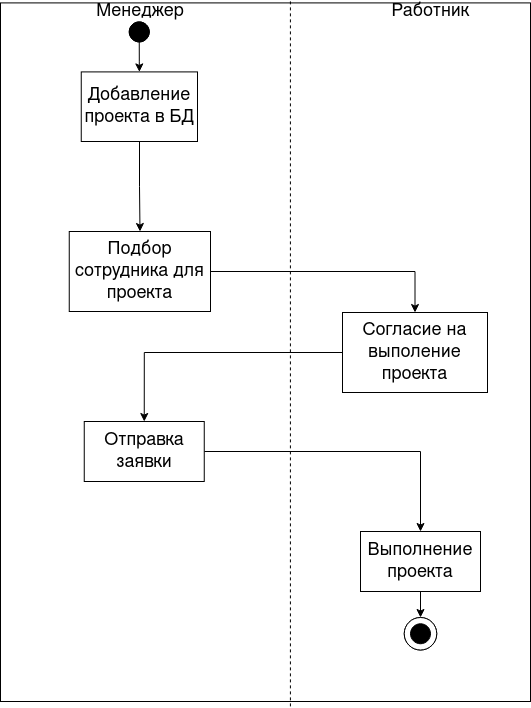
\includegraphics[width=0.4\textwidth]{img/Диаграмма Бизнес-процесса}
\end{FIGURE}
Варианты использования реализуемой системы:
\begin{itemize}
	\item Просмотр активных проектов
	\item Поиск компетенций исполнителя
	\item Подбор сотрудника для проекта
	\item Редактирование информации о исполнителя
\end{itemize}

Так как в данной работе нужно проверить гипотезу, будет разрабатываться прототип программы. Диаграмма вариантов использования конечного программного продукта \ref{fig:figure2}.
\begin{FIGURE}[h]{Диаграмма вариантов использования \label{fig:figure2}}
	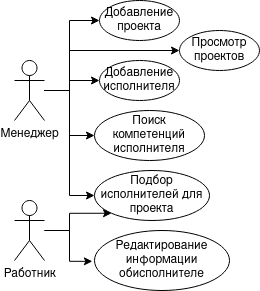
\includegraphics[width=0.4\textwidth]{img/Диаграмма вариантов использования}
\end{FIGURE}

%%%%%%%%%%%%%%%%%%%%%%%%%%
% Расписать прецеденты(?)% 
%%%%%%%%%%%%%%%%%%%%%%%%%%

\section{Выбор языка программирования}
Для прототипирования подходят следующие языки: Python, C\#, Java, JavaScript. Основными критериями для выбора языка были:
\begin{itemize}
	\item Библиотеки для обучения моделей. Для работы с моделями машинного обучения.
	\item Предобученные модели. Так как для обучения модели надо иметь большой объем данных и много вычислительных мощностей.
	\item Библиотека для обработки docx и pdf файлов и обработки сайтов.
	\item Простота написание и отладки программы.
	\item Интерактивный режим.
\end{itemize} 

Под эти критерии подходит Python. Он простой для написание и отладки, так как это интерпретируемый язык программирования, у него есть интерактивный режим. Также есть фреймворк PyThorch и библиотека с предобученными моделями HuggingFace Transformers, в частности RuBERT \cite{kuratov2019adaptation}, а также есть библиотека Bert Extractive Summarizer \cite{miller2019leveraging} для удобной работы с моделей.

\section{Выбор СУБД}
Для Python существуют библиотеки для работы с любыми системами управления базами данных. Для курсовой работы был выбран SQLite потому что его легко настраивать, нет необходимости устанавливать ничего дополнительно, что достаточно для прототипирования с небольшим количеством данных.
\chapter{Проектирование системы}
\section{Проектирование базы данных}
Для хранение информации о преподавателях и выпускных квалификационных работах, где они были руководителями была разработана база данных. Необходимо было хранить:

\begin{description}
	\item [Код преподавателя] -- уникальный код преподавателя
	\item [ФИО преподавателя] -- фамилия имя и отчество преподавателя
	\item [Ссылка на профиль преподавателя] -- ссылка на профиль преподавателя на сайте Высшей школы экономики
	\item [Компетенции] -- полученные компетенции преподавателя
	\item [Эмбеддинги] -- компетенции преподавателя в векторном пространстве
	
	\item [Код ВКР]  -- уникальный код выпускной квалификационной работы
	\item [Название ВКР] -- название выпускной квалификационной работы
	\item [Код преподавателя] -- код преподавателя
	\item [Ссылка на ВКР] -- ссылка на выпускную квалификационную работу на сайте ВШЭ
	\item [Ссылка на полный текст ВКР] -- ссылка на файл для загрузки с полным текстом ВКР
	\item [ФИО студента] -- фамилия имя и отчество студента
	\item [Код ОП студента] -- код образовательной программы студента
	
	\item [Код статуса] -- уникальный код статуса
	\item [Наименования статуса] -- доцент, старший научный сотрудник и тд.
	
	\item [Код кафедры] -- уникальный код кафедры
	\item [Наименование кафедры] -- название кафедры
	
	\item [Код кампуса] -- уникальный код
	\item [Наименования кампуса] -- название кампуса
	
	\item [Код образовательной программы] -- уникальный код
	\item [Код факультета] -- код факультета
	\item [Наименование ОП] -- название образовательной программы
	
	\item [Код факультета] -- уникальный код факультета
	\item [Наименование факультета] -- название факультета
\end{description} 
Описание данных для проектирования БД \ref{tbl:tableDB}.
\begin{TABLE}[!h]{Таблица атрибутов \label{tbl:tableDB}}
	\begin{tabular}[c]{|p{4cm}|l|p{3cm}|l|p{3cm}|}
% longtable не работает
%		\hline Имя атрибута & Тип данных & Значение по умолчанию & Формат ввода & Ограничение на значения \\ \hline
%		\endfirsthead
%		\hline Имя атрибута & Тип данных & Значение по умолчанию & Формат ввода & Ограничение на значения \\ \hline
%		\endhead
%		\hline
%		\endfoot
%		\hline
%		\endlastfoot
		
		\hline
		Имя атрибута & Тип данных & Значение по умолчанию & Формат ввода & Ограничение на значения\\ \hline

		Код преподавателя 				& Число  & Нет & Нет 		& Нет \\ \hline
		ФИО преподавателя 				& Строка & Нет & Нет 		& Нет \\ \hline	
		Ссылка на профиль преподавателя & Строка & Нет & Нет 		& Нет \\ \hline
		Компетенции 					& Строка & Нет & Нет 		& Нет \\ \hline
		Эмбеддинги 						& Число  & Нет & Нет 		& Нет \\ \hline
		Код ВКР 						& Число  & Нет & Нет 		& Нет \\ \hline
		Название ВКР 					& Строка & Нет & Нет 		& Нет \\ \hline
		Ссылка на ВКР 					& Строка & Нет & Нет 		& Нет \\ \hline
		Ссылка на полный текст ВКР 		& Строка & Нет & Нет 		& Нет \\ \hline
		ФИО студента 					& Строка & Нет & Нет 		& Нет \\ \hline
		Код ОП студента 				& Число  & Нет & 00.00.00	& Нет \\ \hline
		Код статуса 					& Число  & Нет & Нет		& Нет \\ \hline
		Наименования статуса 			& Строка & Нет & Нет 		& Нет \\ \hline
		Код кафедры 					& Число  & Нет & Нет 		& Нет \\ \hline
		Наименование кафедры 			& Строка & Нет & Нет 		& Нет \\ \hline
		Код кампуса 					& Число  & Нет & Нет 		& Нет \\ \hline
		Наименования кампуса 			& Строка & Нет & Нет 		& Нет \\ \hline
		Код образовательной программы 	& Число  & Нет & 00.00.00 	& Нет \\ \hline
		Код факультета		 			& Число  & Нет & Нет 		& Нет \\ \hline
		Наименование ОП 				& Строка & Нет & Нет	 	& Нет \\ \hline
		Код факультета 					& Число  & Нет & Нет 		& Нет \\ \hline
		Наименование факультета 		& Строка & Нет & Нет 		& Нет \\ \hline
	\end{tabular}
\end{TABLE}

\subsection{Приведение к 1НФ}
Отношение находится в первой нормальной форме, если выполнены все свойства реляционных отношений, в частности все атрибуты отношения принимают простые значения (атомарные или неделимые), не являющиеся множеством или кортежем из более элементарных составляющих, все кортежи уникальны (отсутствуют дубли).
\begin{enumerate}
	\item \underline{Код преподавателя}
	\item ФИО преподавателя
	\item Ссылка на профиль преподавателя
	\item Компетенции
	\item Эмбеддинги
	\item Код статуса преподавателя
	\item Код кафедры преподавателя
		
	\item \underline{Код ВКР}
	\item Название ВКР
	\item Код преподавателя
	\item Ссылка на ВКР
	\item Ссылка на полный текст ВКР
	\item ФИО студента
	\item Код кампуса
	\item Код ОП студента
	
	\item \underline{Код статуса}
	\item Наименование статуса
	
	\item \underline{Код кафедры}
	\item Наименование кафедры
	
	\item \underline{Код кампуса}
	\item Наименования кампуса
	
	\item \underline{Код образовательной программы}
	\item Код факультета
	\item Наименование ОП
	
	\item \underline{Код факультета}
	\item Наименование факультета
\end{enumerate} 

Данные атрибуты находятся в 1НФ.
\subsection{Приведение к 2НФ}
Отношение находится во второй нормальной форме, если оно находится в первой нормальной форме и каждый неключевой атрибут функционально полно зависит от всего ключа в целом, то есть отсутствует частичная функциональная зависимость не ключевых атрибутов от ключа.
В соответствии с описанными выше зависимостями можно сделать вывод, что в описанном отношении имеются следующие частичные зависимости:
\begin{enumerate}
	\item Код преподавателя определяет:
	\begin{itemize}
		\item ФИО преподавателя
		\item Ссылка на профиль преподавателя
		\item Компетенции
		\item Эмбеддинги
		\item Код статуса преподавателя
		\item Код кафедры преподавателя
	\end{itemize}
	\item Код ВКР определяет:
	\begin{itemize}
		\item Название ВКР
		\item Код преподавателя
		\item Ссылка на ВКР
		\item Ссылка на полный текст ВКР
		\item ФИО студента
		\item Код кампуса
		\item Код ОП студента
	\end{itemize}
	\item Код статуса преподавателя определяет:
	\begin{itemize}
		\item Наименование статуса
	\end{itemize}
	\item Код факультета определяет:
	\begin{itemize}
		\item Наименование факультета
	\end{itemize}
	\item Код кампуса определяет:
	\begin{itemize}
		\item Наименование кампуса
	\end{itemize}
	\item Код кафедры определяет:
	\begin{itemize}
		\item Наименование кафедры
	\end{itemize}
	\item Код образовательной программы определяет:
	\begin{itemize}
		\item Название образовательной программы
	\end{itemize}
\end{enumerate}
\subsection{Приведение к 3НФ}
Отношение находится в третьей нормальной форме, если оно находится во второй нормальной форме, и каждый неключевой атрибут не является транзитивно зависимым от первичного ключа.
\section{Сбор данных}
Для сбора данных надо было обрабатывать страницы сайтов. Для этого использовалась библиотека BeautifulSoap.

В первую очередь надо было получить список преподавателей и ссылки на их страницы. Для этого обрабатывался сайт со списком преподавателей, но там можно получить преподавателей, фамилии которых начинаются на 1 букву. Что бы решить эту проблему с сайты получались ссылки на буквы. А потом с каждой такой ссылки собирался список преподавателей и ссылки на их страницы. Для этого брались все элементы страницы с атрибутом "a"\ и классом "link"\ , в которых значение атрибута "href"\ было "/org/persons/"\ или "/staff/". В базу данных записывались ФИО преподавателя и ссылку на их страницу. 

Далее надо было получить список ВКР для каждого преподавателя. Для этого брались все элементы страницы с атрибутом "a"\ и классом "link"\ , в которых значение атрибута "href"\ было "/edu/vkr/". Итого получилось собрать информацию о 321 преподавателе и 1708 ВКР.

Потом надо было получить информацию о ВКР, но их данные ВКР, в отличие от данных преподавателей, подгружались после загрузки основой страницы. Чтобы решить эту проблему пришлось эмулировать работу браузера с помощью библиотеки Selenium и драйвера Gecko (движок браузера FireFox). Для полной загрузки страницы ставилась задержка в 2 секунды. И бралась информация атрибута "p"\ с классом "vkr-card\_\_item". Также бралась информация о научном руководителе, он искался в базе данных, и потом в базу данных уже записывался Код преподавателя.

Чтобы получить тексты из файлов, они обрабатывались с помощью textract и помещались в базу данных.
\section{Создание профиля человека}
Для создание профиля человека рассматривались TFiDF и суммаризация текста c помощью BERT\cite{devlin2019bert} (Bidirectional Encoder Representations from Transformers). 

Подход TFiDF заключается в том что бы для каждого слова посчитать его отношение числа вхождений некоторого слова к общему числу слов документа (TF) и частоты, с которой некоторое слово встречается в документах коллекции (DF). Данный подход часто используется для кластеризации текстов. Но данный метод плохо подходит для данной задачи, потому что он не рассматривает контекст используемых слов. Это значит у него проблемы с омонимами и синонимами.

BERT рассматривает контекст, в котором находится слово. Каждое слово преобразуется в векторное пространство модели. И модель идет в каждом предложении с лева направо и с право налево пытаясь предсказать, какое будет следующее слово. Для того что бы модель не смотрела в 'будущее' убирается примерно 15\% слов из предложения и модель пытается предсказать, что находится на этом месте.

Для получение компетенций преподавателя использовались тексты ВКР, которые у него писали студенты. Для этого обрабатывался сайты Высшей школы экономики и скачивались тексты ВКР. Потом эти тексты группировались по преподавателю и обрабатывались с помощью BERT Extractive summarizer, в качестве модели для обучения использовался предобученный RuBERT от DeepPavlovAI. 

BERT Extractive summarizer -- использует предпредпоследний слой модели в качестве данных. Потом использует алгоритм K-Means для кластеризации текстов.
\chapter{Поиск человека}

\chapter*{Заключение}
\putbibliography %Вместо этой команды будет вставлена библиография

\chapter*{Приложения}
\end{document}
